\subsection{Classification}
\subsubsection{Simulated AT-TPC events}
Using the \lstinline{RandomSearch} framework we were able to find a network configuration for both the convolutional and DRAW networks that shows very strong performance on the simulated data. Figure \ref{tab:clf_simulated} shows that the strongest performance was obtained using a mean squared error loss function for reconstruction. The fact that one loss function is preferred can be simply argued from the function-shape of the respective losses and aspects of gradient descent. We illustrate this discrepancy in figure \ref{fig:loss_func_shape} where we note that the cross entropy has an asymmetry that punishes higher predictions in a way that is not physically substantiated. As for the strong preference for the maximum mean discrepancy error this can be explained by a rather subtle difference in the objective of the latent loss. As \citet{Antoran2019} shows the mapping of the latent space to an isotropic Gaussian distribution as the Kullback-Leibler objective aims to achieve contributes to the washing out of class information, but strongly encourages feature information. \citet{Antoran2019} describes feature information as e.g stroke thickness or skew when drawing a number, while class information is the more esoteric "five"-ness of all drawings of the number five.

\begin{figure}
\centering
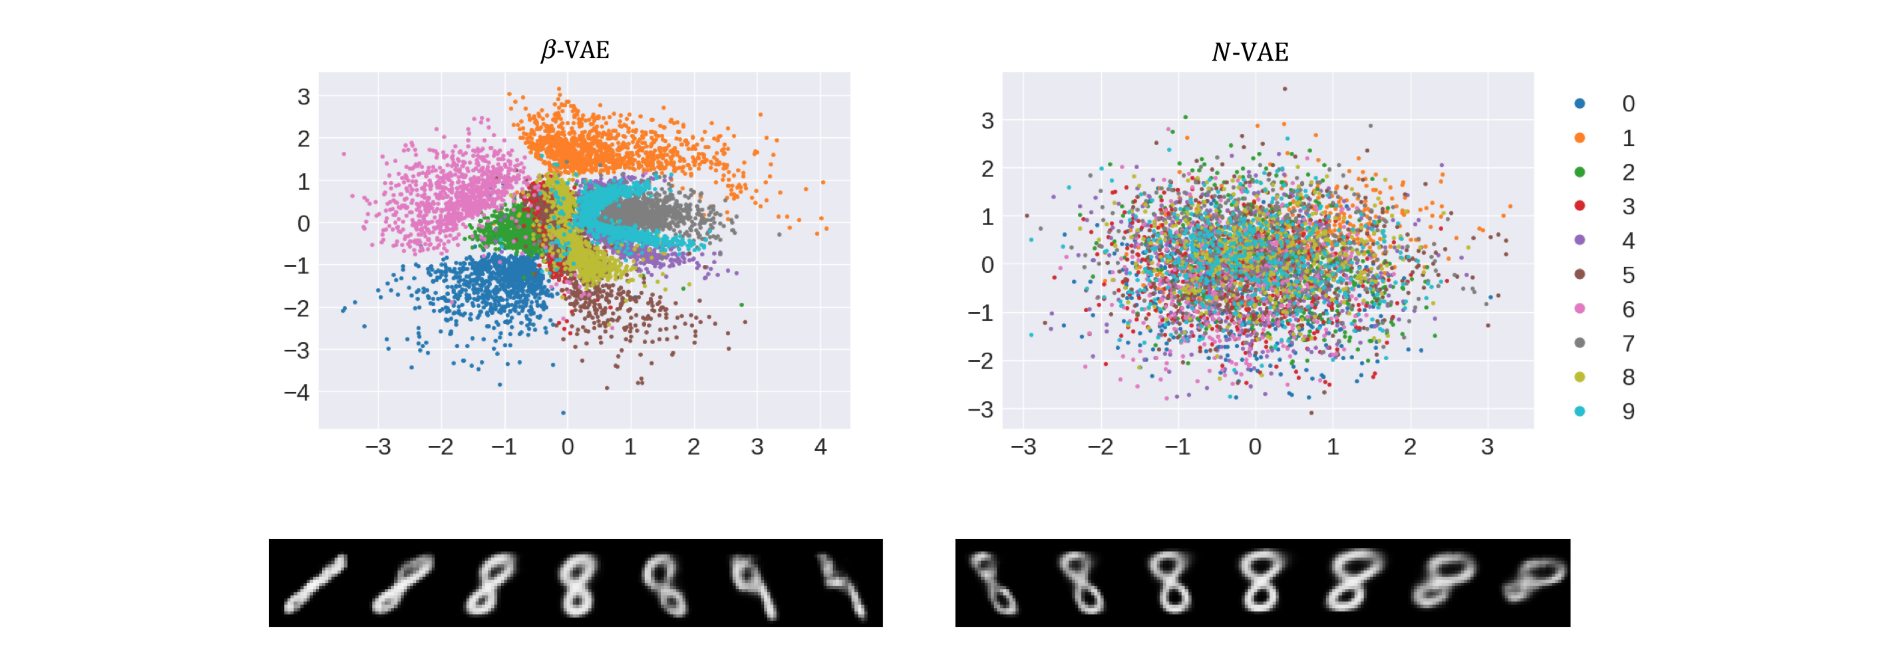
\includegraphics[width=\textwidth, height=3in]{plots/latent_traversal}
\caption{Demonstrating the difference of capturing class and feature information in the latent space. On the left the $\beta$-VAE pushes the autoencoder to a representation favoring encoded class information in the latent space. The spaces between the class blobs makes for a poor generative algorithm, but for the purpose of classification or even clustering this is strongly preferable. On the right the natural clustering of feature information is demonstrated by the convincingly isotropic nature of the latent space distribution. The subplots under the latent distributions demonstrate reconstructions of a traversal along a latent axis, clearly showing the difference between feature and class information. Figure copied from \citet{Antoran2019}}\label{fig:latent_traversal}
\end{figure}

 Indeed this objective works in favor of the variational autoencoder by tightening the distribution, i.e. achieving a density in the latent space without holes, that allows for the generation of new samples without areas in the latent space that do not have a corresponding output. 

\begin{figure}
\centering
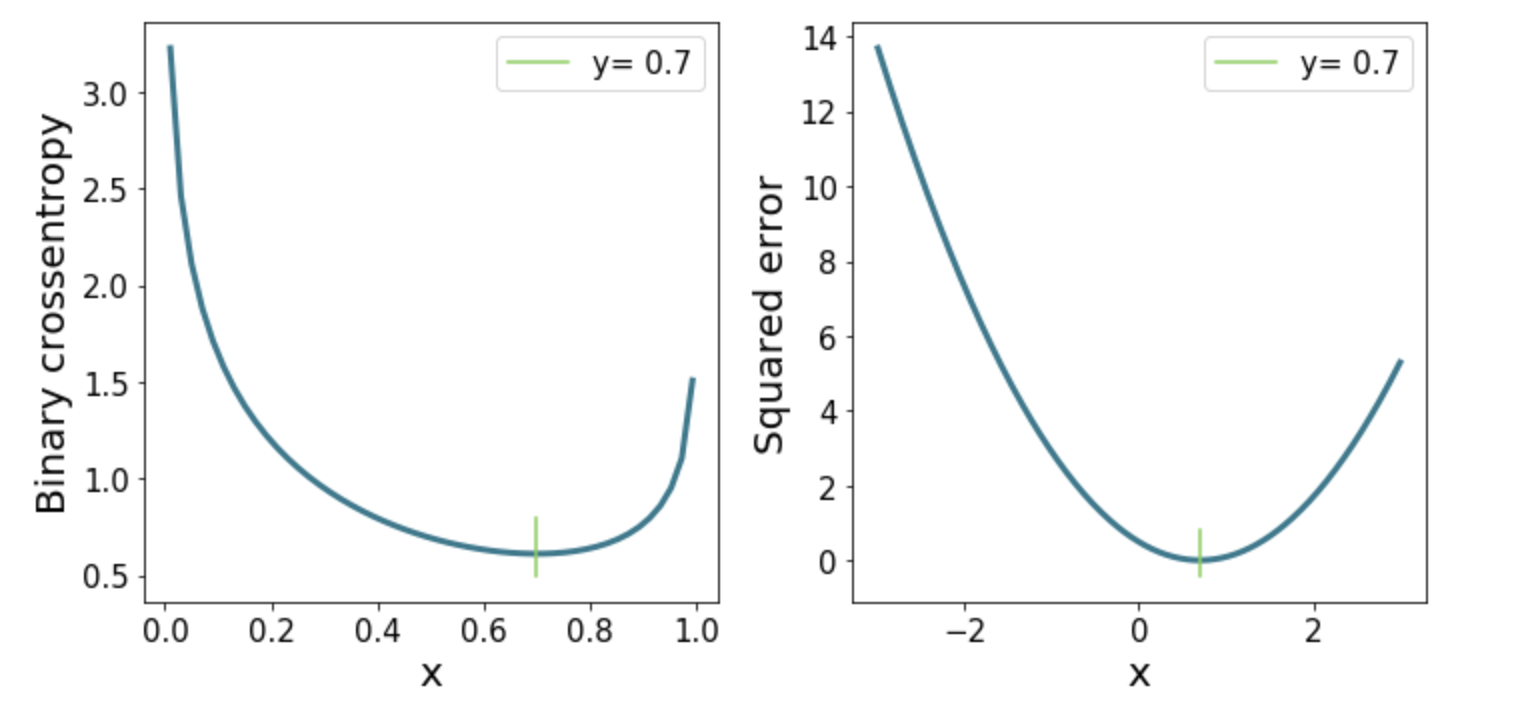
\includegraphics[width=\textwidth]{plots/loss_func_shape.png}
\caption{Illustrating the difference between the function shapes of binary cross-entropy and the mean squared error for the same target value $y=0.7$. We observe that though the two functions have the same minimum the landscape surrounding it is very different. Perhaps most telling is the asymmetry of the cross entropy, implicitly telling the optimizer that values above the targets are measurably worse than those below as measured by the steepness of the gradient. For the AT-TPC data this then implies that predicting higher charge values are worse than predicting lower than the target, and implication that is not physically substantiated}\label{fig:loss_func_shape}
\end{figure}